\section{Activity Diagram}
In der abschließenden Phase des Projekts, wurden die für uns am häufigsten auftretenden Interaktionen zwischen Benutzer und \textit{SmartWatch} als Aktivität dargestellt. Diese sind unserer Ansicht nach, das \textit{Laden der Uhr}, das \textit{Starten von Apps} und die \textit{Telefon -und Mitteilungsfunktionalität}.\\
\begin{figure}[h]
\centering\
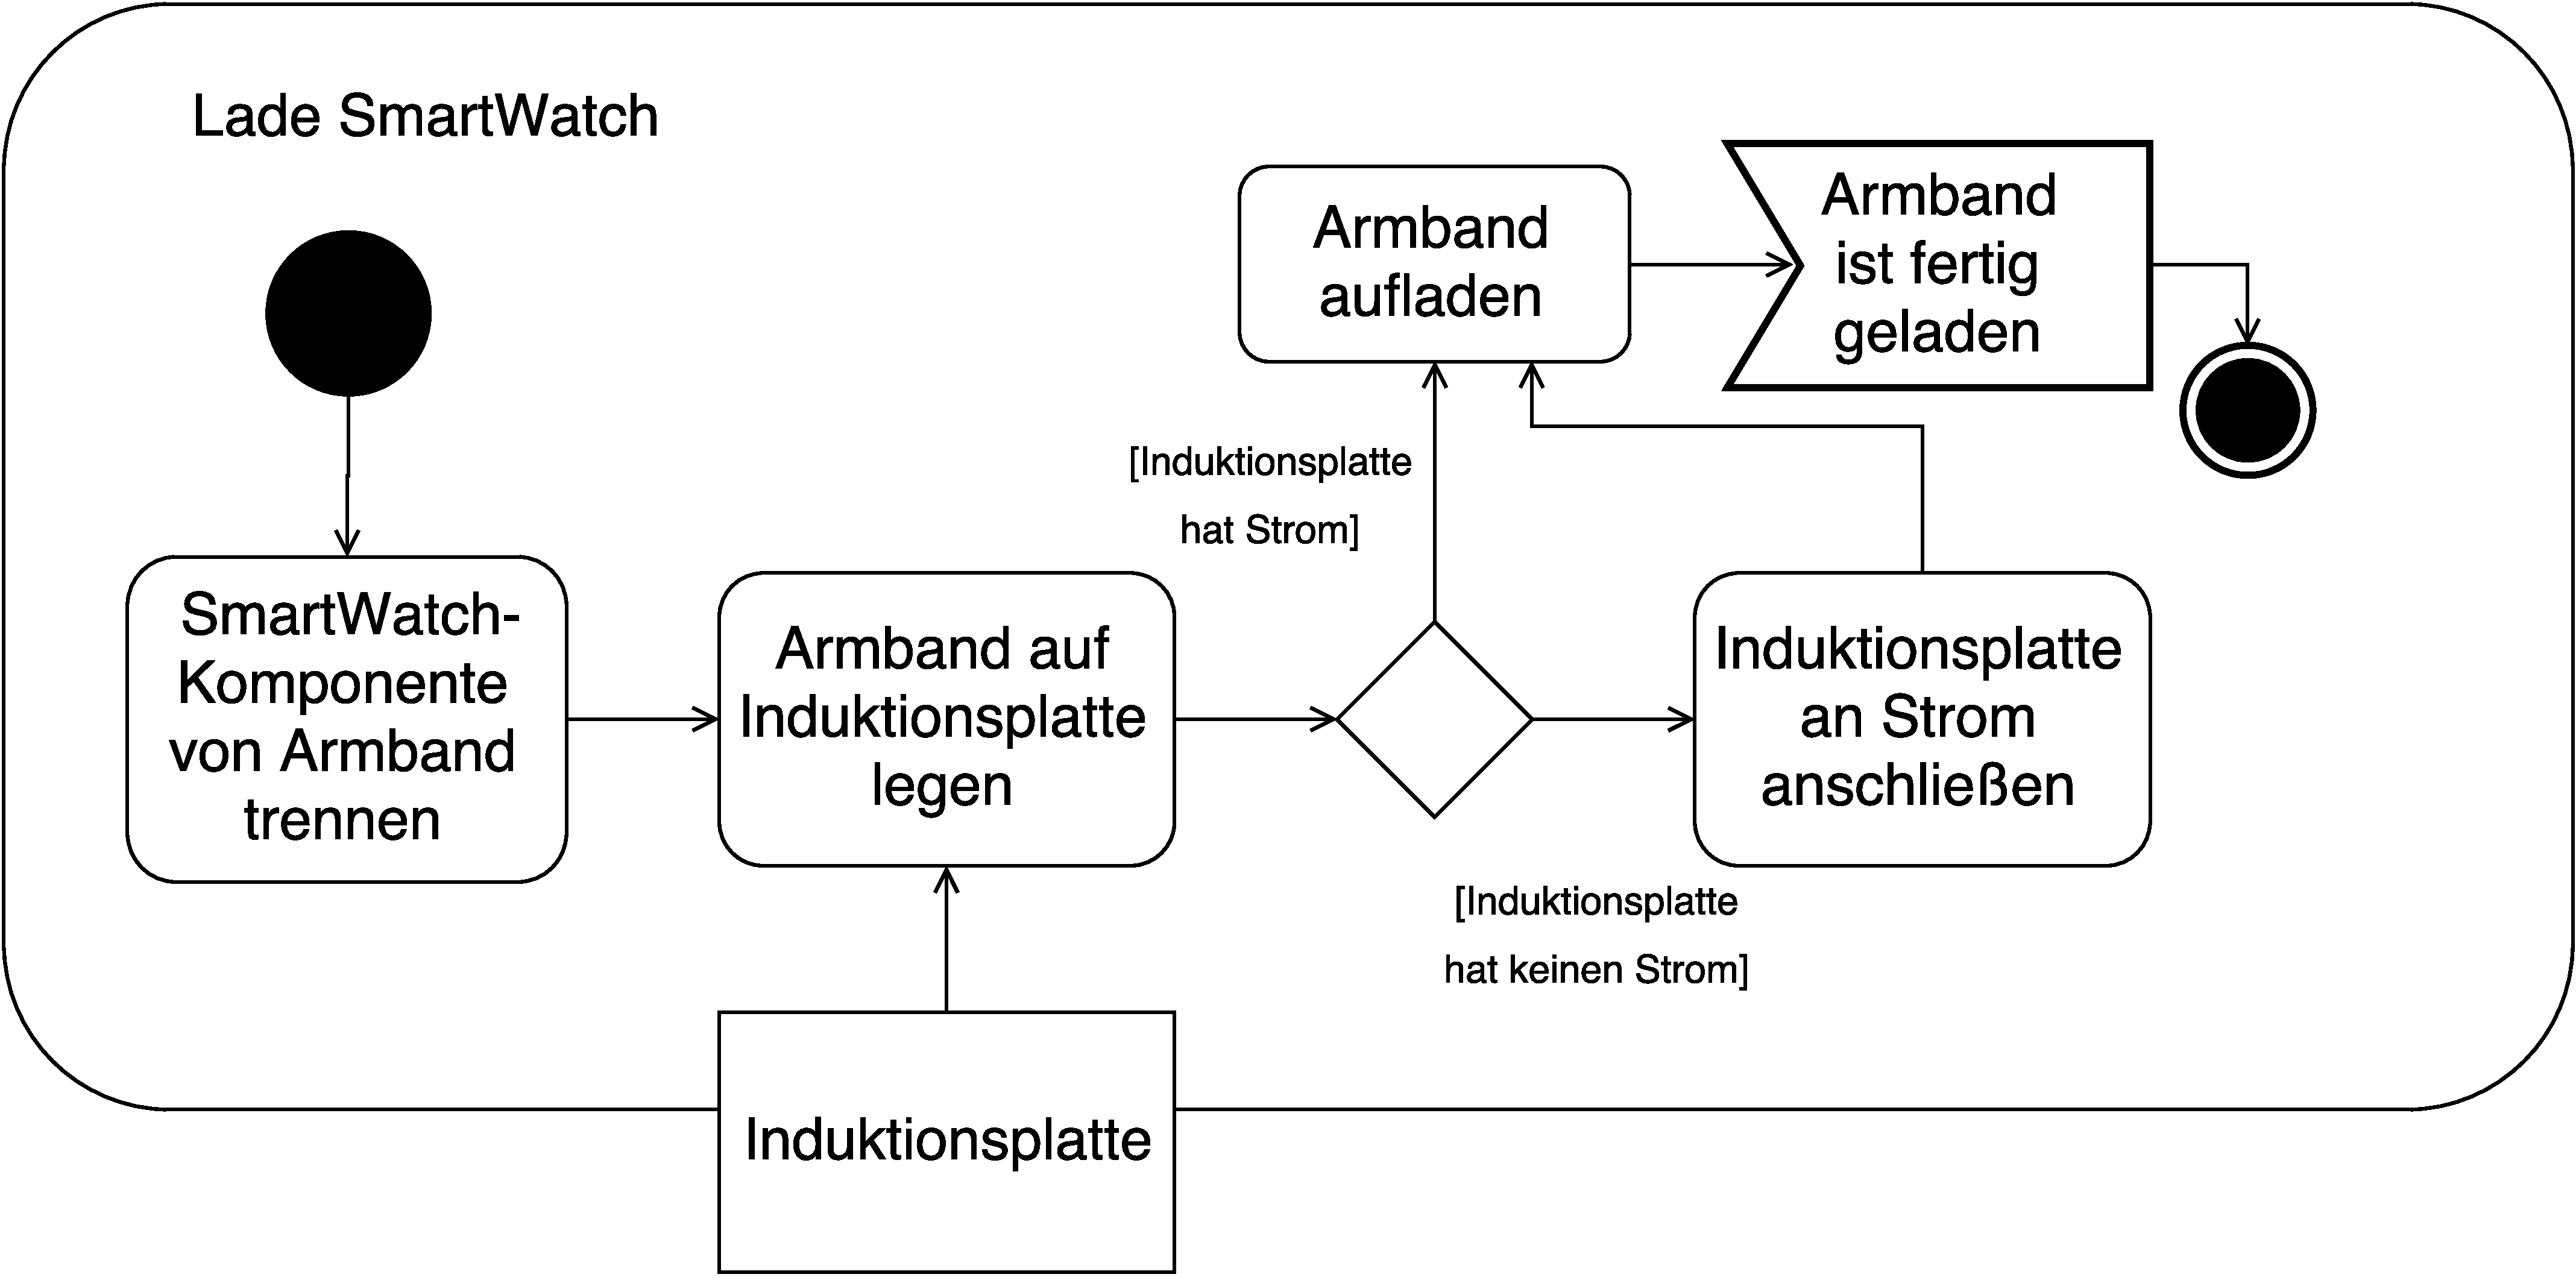
\includegraphics[width=\textwidth]{img/activityLaden}
\caption{Laden des SmartWatch-Armbandes über die mitgelieferte Induktionsplatte.}\label{fig:activityLaden}
\end{figure}
Zunächst betrachten wir den \textit{Ladevorgang} der \textit{SmartWatch} in Abbildung \ref{fig:activityLaden}.
Um die \textit{SmartWatch} laden zu können, muss das \textit{Uhren-Modul} zunächst vom \textit{Armband} getrennt werden. Geladen wird die Uhr per \textit{Induktion} über eine mitgelieferte \textit{Induktionsplatte}. Das \textit{Armband} wird nur geladen, sofern die \textit{Induktionsplatte} am \textit{Stromnetz} angeschlossen wird.\\
\begin{figure}[h]
\centering\
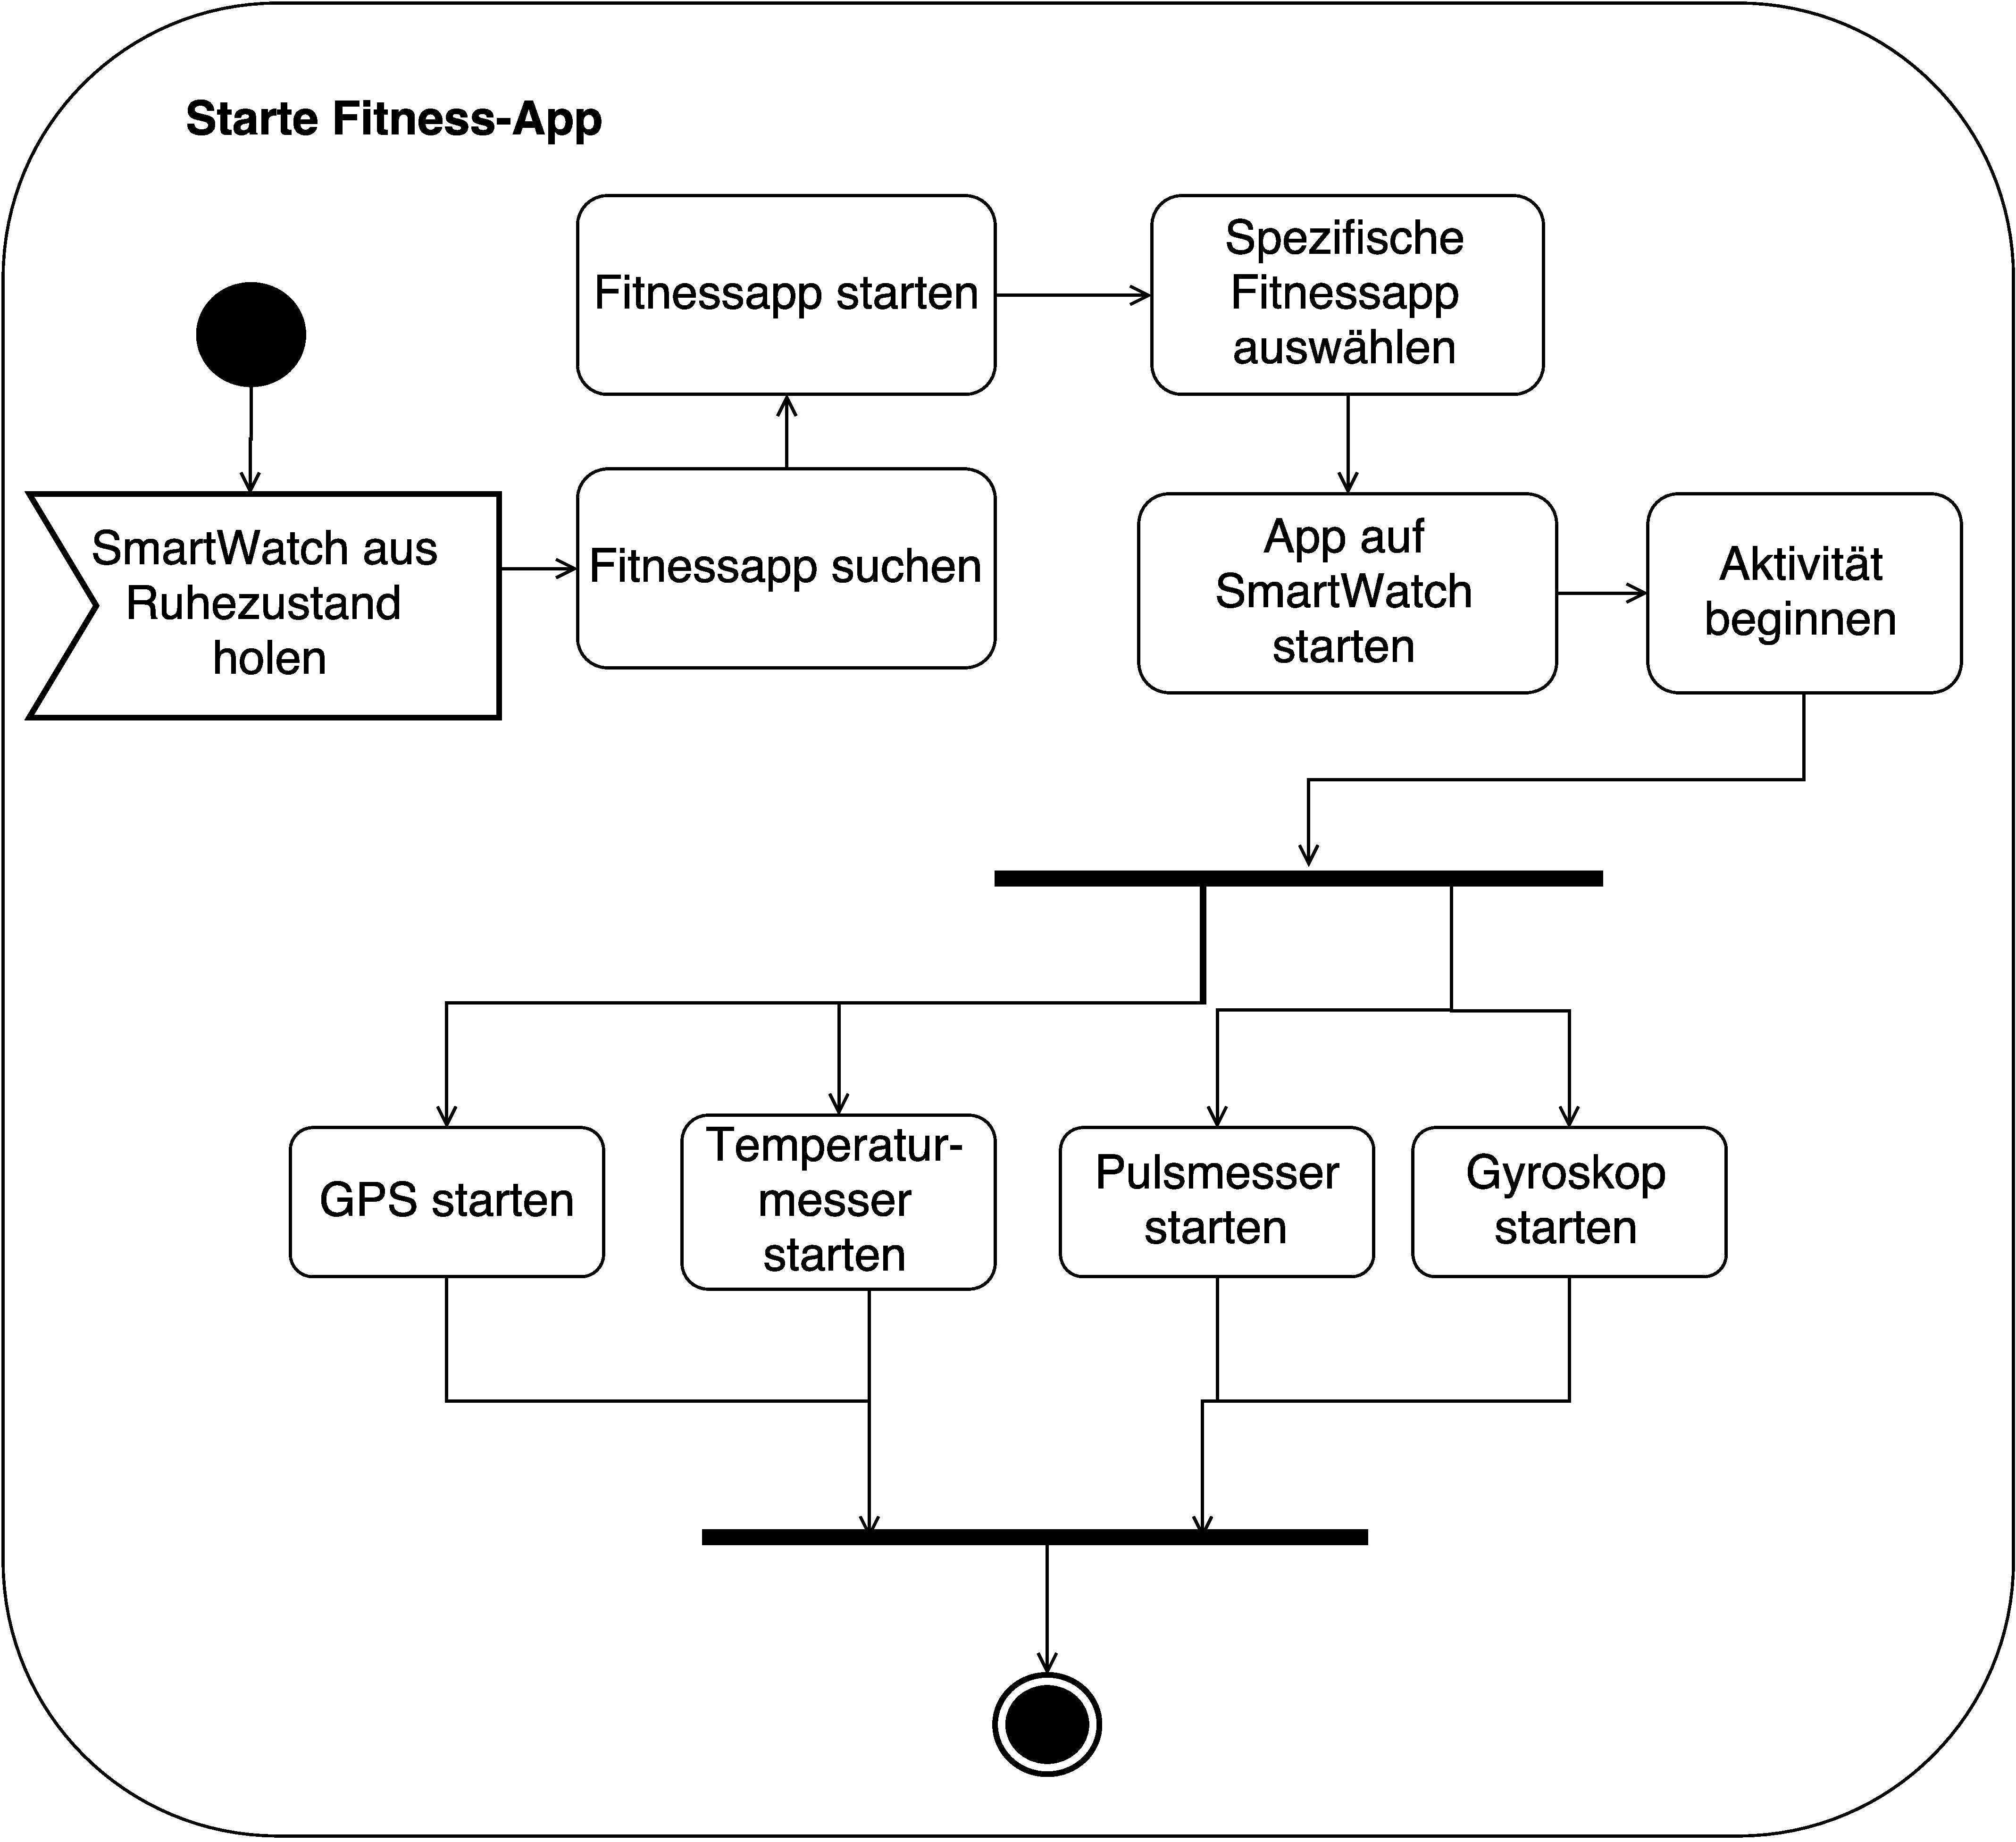
\includegraphics[width=\textwidth]{img/activityFitness}
\caption{Starten einer Fitnessapp durch den Benutzer.}\label{fig:activityFitness}
\end{figure}
Da die \textit{SmartWatch} über \textit{\gls{native} Fitnessapplikationen} verfügt, werden diese anders als die \textit{normalen SmartPhone-Applikationen} gestartet (Abb. \ref{fig:activityFitness}).
Für das Starten einer \textit{Fitnessapplikation} wird die \textit{SmartWatch} zunächst aus dem Ruhezustand geholt. Sobald die \textit{SmartWatch} betriebsbereit ist, kann man über das \textit{Appmenü} die \textit{Fitnessapp} suchen und aktivieren. Daraufhin erscheint eine Liste mit verschiedenen \textit{spezifischen Aktivitäten}, wie z.B. \textit{Laufen} oder \textit{Fahrradfahren}. Sobald die \textit{Aktivität} ausgewählt und gestartet wurde, werden auf der \textit{SmartWatch} das \textit{GPS}, der \textit{Temperatursensor}, der \textit{Pulsmesser}, und das \textit{Gyroskop} aktiviert.\\
Da die \textit{Fitnessfunktionalität} keine Verbindung zum \textit{SmartPhone} erfordert, unterscheidet sich das Starten einer normalen Applikation (Abb. \ref{fig:activityAppKit}). Auch hierfür muss die \textit{SmartWatch} zunächst aus ihrem \textit{Ruhezustand} geholt werden. Zunächst überprüft die \textit{SmartWatch} über das \textit{Appmenü}, ob überhaupt eine Verbindung zum \textit{SmartPhone} besteht, bevor auf dessen \textit{Applikationen} zugegriffen werden kann. Nur bei einer erfolgreichen Verbindung werden die \textit{Programme} des \textit{Telefons} auf der \textit{SmartWatch} angezeigt. Nachdem eine \textit{Applikation} ausgewählt wurde, wird diese zunächst auf dem \textit{SmartPhone} ausgeführt. Über die \textit{Bluetooth-Schnittstelle} lässt sich nun das \textit{Programm} über das \textit{SmartWatch-Interface} steuern.\\
Als Nächstes wird die \textit{Telefonieren} Aktivität betrachtet (Abb. \ref{fig:activityTelefonieren}). Dieses Diagramm beschreibt das Verhalten der \textit{Uhr} bei einem bereits \textit{angenommenen Gespräch}. Hier wird davon ausgegangen, dass bereits eine bestehende Verbindung zwischen \textit{SmartWatch} und \textit{SmartPhone} besteht. Sobald das \textit{Gespräch} begonnen wurde, werden \textbf{parallel} das \textit{Mikrophon} und der \textit{Lautsprecher} der \textit{Uhr} gestartet und mit dem \textit{SmartPhone} synchronisiert. Das bedeutet, dass jeder Spracheingang und Audioausgang, der sonst über das \textit{SmartPhone} stattfinden würde, stattdessen über die \textit{SmartWatch} abgewickelt wird. So können über die \textit{Uhr} \textbf{parallel} \textit{Audiosignale gesendet} und \textit{empfangen} werden. Dies geschieht so lange, bis das \textit{Telefonat} beendet wird. Anschließend werden sowohl \textit{Mikrophon} als auch \textit{Lautsprecher} beendet.\\
Zum Schluss wird betrachtet, was passiert, wenn auf dem \textit{Mobiltelefon} eine \textit{Mitteilung} eingeht (Abb. \ref{fig:activityMitteilung}). Die \textit{empfangene Nachricht} wird, nachdem sie auf dem \textit{SmartPhone} verarbeitet wurde, an die \textit{SmartWatch} weitergeleitet. Sobald die \textit{Uhr} die Nachricht empfangen hat, aktiviert sich die \textit{Displaybeleuchtung} und der \textit{Vibrationsmotor} beginnt sich zu drehen. Anschließend wird der \textit{Nachrichtentext} auf der Uhr ausgegeben. Das Verhalten hierbei kann sich aufgrund verschiedener Einstellungen von Ton und Vibration unterscheiden. Falls der \textit{Benutzer} nach \textbf{15 Sekunden} nicht auf die Nachricht reagiert, versetzt sich die \textit{SmartWatch} wieder in den \textit{Ruhezustand}. Sollte rechtzeitig auf die Nachricht reagiert werden, hat der \textit{Benutzer} die Möglichkeit zu antworten und das \textit{Antwortmenü} zu öffnen. Sobald der \textit{Benutzer} die Mitteilung verfasst hat, wird diese über das \textit{SmartPhone} abgesendet. Daraufhin beendet sich das \textit{Antwortmenü} und die \textit{SmartWatch} geht zurück in den \textit{Ruhezustand}.